\documentclass[man]{apa6}
\usepackage{lmodern}
\usepackage{amssymb,amsmath}
\usepackage{ifxetex,ifluatex}
\usepackage{fixltx2e} % provides \textsubscript
\ifnum 0\ifxetex 1\fi\ifluatex 1\fi=0 % if pdftex
  \usepackage[T1]{fontenc}
  \usepackage[utf8]{inputenc}
\else % if luatex or xelatex
  \ifxetex
    \usepackage{mathspec}
  \else
    \usepackage{fontspec}
  \fi
  \defaultfontfeatures{Ligatures=TeX,Scale=MatchLowercase}
\fi
% use upquote if available, for straight quotes in verbatim environments
\IfFileExists{upquote.sty}{\usepackage{upquote}}{}
% use microtype if available
\IfFileExists{microtype.sty}{%
\usepackage{microtype}
\UseMicrotypeSet[protrusion]{basicmath} % disable protrusion for tt fonts
}{}
\usepackage{hyperref}
\hypersetup{unicode=true,
            pdftitle={EDLD 610 Final Project},
            pdfauthor={Woocheol Kim~\& Jessica Canfield},
            pdfkeywords={sports, NBA, NHL, NFL, MLB},
            pdfborder={0 0 0},
            breaklinks=true}
\urlstyle{same}  % don't use monospace font for urls
\usepackage{color}
\usepackage{fancyvrb}
\newcommand{\VerbBar}{|}
\newcommand{\VERB}{\Verb[commandchars=\\\{\}]}
\DefineVerbatimEnvironment{Highlighting}{Verbatim}{commandchars=\\\{\}}
% Add ',fontsize=\small' for more characters per line
\usepackage{framed}
\definecolor{shadecolor}{RGB}{248,248,248}
\newenvironment{Shaded}{\begin{snugshade}}{\end{snugshade}}
\newcommand{\AlertTok}[1]{\textcolor[rgb]{0.94,0.16,0.16}{#1}}
\newcommand{\AnnotationTok}[1]{\textcolor[rgb]{0.56,0.35,0.01}{\textbf{\textit{#1}}}}
\newcommand{\AttributeTok}[1]{\textcolor[rgb]{0.77,0.63,0.00}{#1}}
\newcommand{\BaseNTok}[1]{\textcolor[rgb]{0.00,0.00,0.81}{#1}}
\newcommand{\BuiltInTok}[1]{#1}
\newcommand{\CharTok}[1]{\textcolor[rgb]{0.31,0.60,0.02}{#1}}
\newcommand{\CommentTok}[1]{\textcolor[rgb]{0.56,0.35,0.01}{\textit{#1}}}
\newcommand{\CommentVarTok}[1]{\textcolor[rgb]{0.56,0.35,0.01}{\textbf{\textit{#1}}}}
\newcommand{\ConstantTok}[1]{\textcolor[rgb]{0.00,0.00,0.00}{#1}}
\newcommand{\ControlFlowTok}[1]{\textcolor[rgb]{0.13,0.29,0.53}{\textbf{#1}}}
\newcommand{\DataTypeTok}[1]{\textcolor[rgb]{0.13,0.29,0.53}{#1}}
\newcommand{\DecValTok}[1]{\textcolor[rgb]{0.00,0.00,0.81}{#1}}
\newcommand{\DocumentationTok}[1]{\textcolor[rgb]{0.56,0.35,0.01}{\textbf{\textit{#1}}}}
\newcommand{\ErrorTok}[1]{\textcolor[rgb]{0.64,0.00,0.00}{\textbf{#1}}}
\newcommand{\ExtensionTok}[1]{#1}
\newcommand{\FloatTok}[1]{\textcolor[rgb]{0.00,0.00,0.81}{#1}}
\newcommand{\FunctionTok}[1]{\textcolor[rgb]{0.00,0.00,0.00}{#1}}
\newcommand{\ImportTok}[1]{#1}
\newcommand{\InformationTok}[1]{\textcolor[rgb]{0.56,0.35,0.01}{\textbf{\textit{#1}}}}
\newcommand{\KeywordTok}[1]{\textcolor[rgb]{0.13,0.29,0.53}{\textbf{#1}}}
\newcommand{\NormalTok}[1]{#1}
\newcommand{\OperatorTok}[1]{\textcolor[rgb]{0.81,0.36,0.00}{\textbf{#1}}}
\newcommand{\OtherTok}[1]{\textcolor[rgb]{0.56,0.35,0.01}{#1}}
\newcommand{\PreprocessorTok}[1]{\textcolor[rgb]{0.56,0.35,0.01}{\textit{#1}}}
\newcommand{\RegionMarkerTok}[1]{#1}
\newcommand{\SpecialCharTok}[1]{\textcolor[rgb]{0.00,0.00,0.00}{#1}}
\newcommand{\SpecialStringTok}[1]{\textcolor[rgb]{0.31,0.60,0.02}{#1}}
\newcommand{\StringTok}[1]{\textcolor[rgb]{0.31,0.60,0.02}{#1}}
\newcommand{\VariableTok}[1]{\textcolor[rgb]{0.00,0.00,0.00}{#1}}
\newcommand{\VerbatimStringTok}[1]{\textcolor[rgb]{0.31,0.60,0.02}{#1}}
\newcommand{\WarningTok}[1]{\textcolor[rgb]{0.56,0.35,0.01}{\textbf{\textit{#1}}}}
\usepackage{graphicx}
% grffile has become a legacy package: https://ctan.org/pkg/grffile
\IfFileExists{grffile.sty}{%
\usepackage{grffile}
}{}
\makeatletter
\def\maxwidth{\ifdim\Gin@nat@width>\linewidth\linewidth\else\Gin@nat@width\fi}
\def\maxheight{\ifdim\Gin@nat@height>\textheight\textheight\else\Gin@nat@height\fi}
\makeatother
% Scale images if necessary, so that they will not overflow the page
% margins by default, and it is still possible to overwrite the defaults
% using explicit options in \includegraphics[width, height, ...]{}
\setkeys{Gin}{width=\maxwidth,height=\maxheight,keepaspectratio}
\IfFileExists{parskip.sty}{%
\usepackage{parskip}
}{% else
\setlength{\parindent}{0pt}
\setlength{\parskip}{6pt plus 2pt minus 1pt}
}
\setlength{\emergencystretch}{3em}  % prevent overfull lines
\providecommand{\tightlist}{%
  \setlength{\itemsep}{0pt}\setlength{\parskip}{0pt}}
\setcounter{secnumdepth}{0}
% Redefines (sub)paragraphs to behave more like sections
\ifx\paragraph\undefined\else
\let\oldparagraph\paragraph
\renewcommand{\paragraph}[1]{\oldparagraph{#1}\mbox{}}
\fi
\ifx\subparagraph\undefined\else
\let\oldsubparagraph\subparagraph
\renewcommand{\subparagraph}[1]{\oldsubparagraph{#1}\mbox{}}
\fi

%%% Use protect on footnotes to avoid problems with footnotes in titles
\let\rmarkdownfootnote\footnote%
\def\footnote{\protect\rmarkdownfootnote}


  \title{EDLD 610 Final Project}
    \author{Woocheol Kim\textsuperscript{1}~\& Jessica Canfield\textsuperscript{1}}
    \date{}
  
\shorttitle{Exploring Trends in Major League Sports }
\affiliation{
\vspace{0.5cm}
\textsuperscript{1} University of Oregon}
\keywords{sports, NBA, NHL, NFL, MLB\newline\indent Word count: X}
\usepackage{csquotes}
\usepackage{upgreek}
\captionsetup{font=singlespacing,justification=justified}

\usepackage{longtable}
\usepackage{lscape}
\usepackage{multirow}
\usepackage{tabularx}
\usepackage[flushleft]{threeparttable}
\usepackage{threeparttablex}

\newenvironment{lltable}{\begin{landscape}\begin{center}\begin{ThreePartTable}}{\end{ThreePartTable}\end{center}\end{landscape}}

\makeatletter
\newcommand\LastLTentrywidth{1em}
\newlength\longtablewidth
\setlength{\longtablewidth}{1in}
\newcommand{\getlongtablewidth}{\begingroup \ifcsname LT@\roman{LT@tables}\endcsname \global\longtablewidth=0pt \renewcommand{\LT@entry}[2]{\global\advance\longtablewidth by ##2\relax\gdef\LastLTentrywidth{##2}}\@nameuse{LT@\roman{LT@tables}} \fi \endgroup}


\DeclareDelayedFloatFlavor{ThreePartTable}{table}
\DeclareDelayedFloatFlavor{lltable}{table}
\DeclareDelayedFloatFlavor*{longtable}{table}
\makeatletter
\renewcommand{\efloat@iwrite}[1]{\immediate\expandafter\protected@write\csname efloat@post#1\endcsname{}}
\makeatother
\usepackage{lineno}

\linenumbers

\authornote{Jessica Canfield \& Woocheol Kim are both Marketing PhD students at the University of Oregon.

Correspondence concerning this article should be addressed to Woocheol Kim, 1208 University St, Eugene, OR 97403. E-mail: \href{mailto:wkim4@uoregon.edu}{\nolinkurl{wkim4@uoregon.edu}}}

\abstract{
One or two sentences providing a \textbf{basic introduction} to the field, comprehensible to a scientist in any discipline.

Two to three sentences of \textbf{more detailed background}, comprehensible to scientists in related disciplines.

One sentence clearly stating the \textbf{general problem} being addressed by this particular study.

One sentence summarizing the main result (with the words ``\textbf{here we show}'' or their equivalent).

Two or three sentences explaining what the \textbf{main result} reveals in direct comparison to what was thought to be the case previously, or how the main result adds to previous knowledge.

One or two sentences to put the results into a more \textbf{general context}.

Two or three sentences to provide a \textbf{broader perspective}, readily comprehensible to a scientist in any discipline.


}

\begin{document}
\maketitle

\begin{Shaded}
\begin{Highlighting}[]
\NormalTok{mlb <-}\StringTok{ }\KeywordTok{import}\NormalTok{(}\KeywordTok{here}\NormalTok{(}\StringTok{"Data"}\NormalTok{, }\StringTok{"MLB.xlsx"}\NormalTok{)) }\OperatorTok
\StringTok{  }\KeywordTok{characterize}\NormalTok{() }\OperatorTok\StringTok{  }
\StringTok{  }\KeywordTok{clean_names}\NormalTok{() }\OperatorTok\StringTok{ }
\StringTok{  }\KeywordTok{select}\NormalTok{(sport, team, year, capacity, attend_tot, attend_avg, games, ticket_price, home_wins) }\OperatorTok\StringTok{ }
\StringTok{  }\KeywordTok{as_tibble}\NormalTok{()  }\OperatorTok\StringTok{ }
\StringTok{  }\KeywordTok{mutate}\NormalTok{(}\DataTypeTok{attend_tot =} \KeywordTok{as.numeric}\NormalTok{(attend_tot),}
         \DataTypeTok{attend_avg =} \KeywordTok{as.numeric}\NormalTok{(attend_avg), }
         \DataTypeTok{capacity =} \KeywordTok{as.numeric}\NormalTok{(capacity), }
         \DataTypeTok{games =} \KeywordTok{as.numeric}\NormalTok{(games), }
         \DataTypeTok{ticket_price =} \KeywordTok{as.numeric}\NormalTok{(ticket_price),}
         \DataTypeTok{home_wins =} \KeywordTok{as.numeric}\NormalTok{(home_wins)) }\CommentTok{#changed attent_tot, games, home_wins, ticket price and attend_avg to numeric to try to get bind to work, also the 'numeric' code gave me an error, I assumed that we wanted this variable to be numeric so I changed it to 'as.numeric' + combined it with the other mutates :) }
\KeywordTok{str}\NormalTok{(mlb) }\CommentTok{#I added code to see the structure of each sports dataset when I was trying to figure out why it wouldn't bind, feel free to remove! }
\end{Highlighting}
\end{Shaded}

\begin{verbatim}
## Classes 'tbl_df', 'tbl' and 'data.frame':    528 obs. of  9 variables:
##  $ sport       : chr  "MLB" "MLB" "MLB" "MLB" ...
##  $ team        : chr  "(Anaheim) Angels" "(Anaheim) Angels" "(Anaheim) Angels" "(Anaheim) Angels" ...
##  $ year        : num  2000 2001 2002 2003 2004 ...
##  $ capacity    : num  65000 65000 65000 45050 45050 ...
##  $ attend_tot  : num  2066977 2000919 2305565 3061094 3375677 ...
##  $ attend_avg  : num  25118 24702 28463 37791 41675 ...
##  $ games       : num  81 81 81 82 81 81 81 81 81 81 ...
##  $ ticket_price: num  13.2 13.4 11.8 16 16.6 ...
##  $ home_wins   : num  46 39 54 45 45 49 45 54 50 49 ...
\end{verbatim}

\begin{Shaded}
\begin{Highlighting}[]
\KeywordTok{is.character}\NormalTok{(mlb}\OperatorTok{$}\NormalTok{capacity) }
\end{Highlighting}
\end{Shaded}

\begin{verbatim}
## [1] FALSE
\end{verbatim}

\begin{Shaded}
\begin{Highlighting}[]
\NormalTok{nba <-}\StringTok{ }\KeywordTok{import}\NormalTok{(}\KeywordTok{here}\NormalTok{(}\StringTok{"Data"}\NormalTok{, }\StringTok{"NBA.xlsx"}\NormalTok{)) }\OperatorTok
\StringTok{  }\KeywordTok{characterize}\NormalTok{() }\OperatorTok\StringTok{  }
\StringTok{  }\KeywordTok{clean_names}\NormalTok{()}\OperatorTok\StringTok{ }
\StringTok{  }\KeywordTok{select}\NormalTok{(sport, team, year, capacity, attend_tot, attend_avg, games, ticket_price, home_win)}\OperatorTok\StringTok{ }
\StringTok{  }\KeywordTok{as_tibble}\NormalTok{() }\OperatorTok\StringTok{ }
\StringTok{  }\KeywordTok{rename}\NormalTok{(}\DataTypeTok{home_wins =}\NormalTok{ home_win) }\OperatorTok\StringTok{ }
\StringTok{  }\KeywordTok{as_tibble}\NormalTok{()}

\NormalTok{nba <-}\StringTok{ }\NormalTok{nba }\OperatorTok\StringTok{ }\KeywordTok{mutate}\NormalTok{(}\DataTypeTok{capacity =} \KeywordTok{as.numeric}\NormalTok{(capacity), }\DataTypeTok{attend_tot =} \KeywordTok{as.numeric}\NormalTok{(attend_tot), }\DataTypeTok{attend_avg =} \KeywordTok{as.numeric}\NormalTok{(attend_avg), }\DataTypeTok{games =} \KeywordTok{as.numeric}\NormalTok{(games), }\DataTypeTok{ticket_price =} \KeywordTok{as.numeric}\NormalTok{(ticket_price), }\DataTypeTok{home_wins =} \KeywordTok{as.numeric}\NormalTok{(home_wins))}
\KeywordTok{str}\NormalTok{(nba)}
\end{Highlighting}
\end{Shaded}

\begin{verbatim}
## Classes 'tbl_df', 'tbl' and 'data.frame':    480 obs. of  9 variables:
##  $ sport       : chr  "NBA" "NBA" "NBA" "NBA" ...
##  $ team        : chr  "Hawks" "Hawks" "Hawks" "Hawks" ...
##  $ year        : num  2000 2001 2002 2003 2004 ...
##  $ capacity    : num  19445 19445 19445 19445 19445 ...
##  $ attend_tot  : num  560324 506110 528644 565728 586390 ...
##  $ attend_avg  : num  13666 12344 12894 13798 14302 ...
##  $ games       : num  41 41 41 41 41 41 41 41 41 41 ...
##  $ ticket_price: num  45.9 42.8 37.5 37.5 37.7 ...
##  $ home_wins   : num  18 23 26 18 9 18 18 25 31 34 ...
\end{verbatim}

\begin{Shaded}
\begin{Highlighting}[]
\NormalTok{ncaaf <-}\StringTok{ }\KeywordTok{import}\NormalTok{(}\KeywordTok{here}\NormalTok{(}\StringTok{"Data"}\NormalTok{, }\StringTok{"NCAAF.xlsx"}\NormalTok{)) }\OperatorTok
\StringTok{  }\KeywordTok{characterize}\NormalTok{() }\OperatorTok\StringTok{  }
\StringTok{  }\KeywordTok{clean_names}\NormalTok{() }\OperatorTok\StringTok{ }
\StringTok{  }\KeywordTok{select}\NormalTok{(sport, team, year, capacity, attend_tot, attend_avg, games, ticket_price, home_wins) }\OperatorTok\StringTok{ }
\StringTok{  }\KeywordTok{as_tibble}\NormalTok{()}
\KeywordTok{str}\NormalTok{(ncaaf)}
\end{Highlighting}
\end{Shaded}

\begin{verbatim}
## Classes 'tbl_df', 'tbl' and 'data.frame':    2064 obs. of  9 variables:
##  $ sport       : chr  "NCAAF" "NCAAF" "NCAAF" "NCAAF" ...
##  $ team        : chr  "Air Force" "Air Force" "Air Force" "Air Force" ...
##  $ year        : num  2000 2001 2002 2003 2004 ...
##  $ capacity    : num  52480 52480 52480 52480 52480 ...
##  $ attend_tot  : num  255357 230631 298993 235259 266302 ...
##  $ attend_avg  : num  42560 38439 42713 39210 38043 ...
##  $ games       : num  6 6 7 6 7 ...
##  $ ticket_price: logi  NA NA NA NA NA NA ...
##  $ home_wins   : num  NA NA NA NA NA NA NA NA NA NA ...
\end{verbatim}

\begin{Shaded}
\begin{Highlighting}[]
\NormalTok{nfl <-}\StringTok{ }\KeywordTok{import}\NormalTok{(}\KeywordTok{here}\NormalTok{(}\StringTok{"Data"}\NormalTok{, }\StringTok{"NFL.xlsx"}\NormalTok{)) }\OperatorTok
\StringTok{  }\KeywordTok{characterize}\NormalTok{() }\OperatorTok\StringTok{  }
\StringTok{  }\KeywordTok{clean_names}\NormalTok{()}\OperatorTok\StringTok{ }
\StringTok{  }\KeywordTok{select}\NormalTok{(sport, team, year, capacity, attend_tot, attend_avg, games, ticket_price, home_wins) }\OperatorTok\StringTok{ }
\StringTok{  }\KeywordTok{as_tibble}\NormalTok{()}

\NormalTok{nfl <-}\StringTok{ }\NormalTok{nfl }\OperatorTok\StringTok{ }\KeywordTok{mutate}\NormalTok{(}\DataTypeTok{attend_tot =} \KeywordTok{as.numeric}\NormalTok{(attend_tot),  }\DataTypeTok{attend_avg =} \KeywordTok{as.numeric}\NormalTok{(attend_avg),}\DataTypeTok{games =} \KeywordTok{as.numeric}\NormalTok{(games), }\DataTypeTok{ticket_price =} \KeywordTok{as.numeric}\NormalTok{(ticket_price), }\DataTypeTok{home_wins =} \KeywordTok{as.numeric}\NormalTok{(home_wins))}
\KeywordTok{str}\NormalTok{(nfl)}
\end{Highlighting}
\end{Shaded}

\begin{verbatim}
## Classes 'tbl_df', 'tbl' and 'data.frame':    528 obs. of  9 variables:
##  $ sport       : chr  "NFL" "NFL" "NFL" "NFL" ...
##  $ team        : chr  "Arizona Cardinals" "Arizona Cardinals" "Arizona Cardinals" "Arizona Cardinals" ...
##  $ year        : num  2000 2001 2002 2003 2004 ...
##  $ capacity    : num  73379 73379 73379 NA 71706 ...
##  $ attend_tot  : num  387475 307315 327272 288499 300267 ...
##  $ attend_avg  : num  NA NA NA NA NA ...
##  $ games       : num  8 8 8 8 8 8 8 8 8 8 ...
##  $ ticket_price: num  39.6 37.6 33.7 36 39.7 ...
##  $ home_wins   : num  3 3 3 4 5 3 3 6 6 4 ...
\end{verbatim}

\begin{Shaded}
\begin{Highlighting}[]
\NormalTok{nhl <-}\StringTok{ }\KeywordTok{import}\NormalTok{(}\KeywordTok{here}\NormalTok{(}\StringTok{"Data"}\NormalTok{, }\StringTok{"NHL.xlsx"}\NormalTok{)) }\OperatorTok
\StringTok{  }\KeywordTok{characterize}\NormalTok{() }\OperatorTok\StringTok{  }
\StringTok{  }\KeywordTok{clean_names}\NormalTok{()}\OperatorTok\StringTok{ }
\StringTok{  }\KeywordTok{select}\NormalTok{(sport, team, year, capacity, attend_tot, attend_avg, games, ticket_price, home_wins) }\OperatorTok\StringTok{ }
\StringTok{  }\KeywordTok{as_tibble}\NormalTok{() }
\KeywordTok{str}\NormalTok{(nhl)}
\end{Highlighting}
\end{Shaded}

\begin{verbatim}
## Classes 'tbl_df', 'tbl' and 'data.frame':    480 obs. of  9 variables:
##  $ sport       : chr  "NHL" "NHL" "NHL" "NHL" ...
##  $ team        : chr  "Ducks" "Ducks" "Ducks" "Ducks" ...
##  $ year        : num  2000 2001 2002 2003 2004 ...
##  $ capacity    : num  17174 17174 17174 17174 17174 ...
##  $ attend_tot  : chr  "553470" "492089" "573524" "614476" ...
##  $ attend_avg  : chr  "13499" "12002" "13998" "14987" ...
##  $ games       : num  41 41 41 41 0 41 41 41 41 41 ...
##  $ ticket_price: chr  "N/A" "N/A" "N/A" "N/A" ...
##  $ home_wins   : num  15 15 22 19 0 26 26 28 20 25 ...
\end{verbatim}

\begin{Shaded}
\begin{Highlighting}[]
\NormalTok{nhl <-}\StringTok{ }\NormalTok{nhl }\OperatorTok\StringTok{ }\KeywordTok{mutate}\NormalTok{(}\DataTypeTok{attend_tot =} \KeywordTok{as.numeric}\NormalTok{(attend_tot), }\DataTypeTok{attend_avg =} \KeywordTok{as.numeric}\NormalTok{(attend_avg), }\DataTypeTok{games =} \KeywordTok{as.numeric}\NormalTok{(games), }\DataTypeTok{ticket_price =} \KeywordTok{as.numeric}\NormalTok{(ticket_price), }\DataTypeTok{home_wins =} \KeywordTok{as.numeric}\NormalTok{(home_wins))}

\NormalTok{sports <-}\StringTok{ }\KeywordTok{bind_rows}\NormalTok{(mlb, nba, ncaaf, nfl, nhl) }\OperatorTok\StringTok{ }\KeywordTok{as_tibble}\NormalTok{()}
\KeywordTok{str}\NormalTok{(mlb)}
\end{Highlighting}
\end{Shaded}

\begin{verbatim}
## Classes 'tbl_df', 'tbl' and 'data.frame':    528 obs. of  9 variables:
##  $ sport       : chr  "MLB" "MLB" "MLB" "MLB" ...
##  $ team        : chr  "(Anaheim) Angels" "(Anaheim) Angels" "(Anaheim) Angels" "(Anaheim) Angels" ...
##  $ year        : num  2000 2001 2002 2003 2004 ...
##  $ capacity    : num  65000 65000 65000 45050 45050 ...
##  $ attend_tot  : num  2066977 2000919 2305565 3061094 3375677 ...
##  $ attend_avg  : num  25118 24702 28463 37791 41675 ...
##  $ games       : num  81 81 81 82 81 81 81 81 81 81 ...
##  $ ticket_price: num  13.2 13.4 11.8 16 16.6 ...
##  $ home_wins   : num  46 39 54 45 45 49 45 54 50 49 ...
\end{verbatim}

\begin{Shaded}
\begin{Highlighting}[]
\NormalTok{sports_rev <-}\StringTok{ }\NormalTok{sports }\OperatorTok
\StringTok{  }\KeywordTok{drop_na}\NormalTok{() }\OperatorTok
\StringTok{  }\KeywordTok{filter}\NormalTok{(year }\OperatorTok{>=}\StringTok{ }\DecValTok{2010}\NormalTok{) }\OperatorTok
\StringTok{  }\KeywordTok{group_by}\NormalTok{(team, sport) }\OperatorTok
\StringTok{  }\KeywordTok{summarize}\NormalTok{(}\DataTypeTok{avg_ticket_price =} \KeywordTok{mean}\NormalTok{(ticket_price), }\DataTypeTok{avg_homewins =} \KeywordTok{mean}\NormalTok{(home_wins), }\DataTypeTok{avg_attendance =} \KeywordTok{mean}\NormalTok{(attend_avg)) }

\NormalTok{sports_rev }\OperatorTok
\StringTok{  }\KeywordTok{ggplot}\NormalTok{(}\KeywordTok{aes}\NormalTok{(avg_ticket_price, avg_attendance, }\DataTypeTok{color =}\NormalTok{ sport)) }\OperatorTok{+}
\StringTok{  }\KeywordTok{geom_point}\NormalTok{() }\OperatorTok{+}
\StringTok{  }\KeywordTok{geom_smooth}\NormalTok{(}\DataTypeTok{method =}\NormalTok{ lm, }\DataTypeTok{se =} \OtherTok{FALSE}\NormalTok{) }\OperatorTok{+}\StringTok{ }
\StringTok{  }\KeywordTok{theme_minimal}\NormalTok{()}
\end{Highlighting}
\end{Shaded}

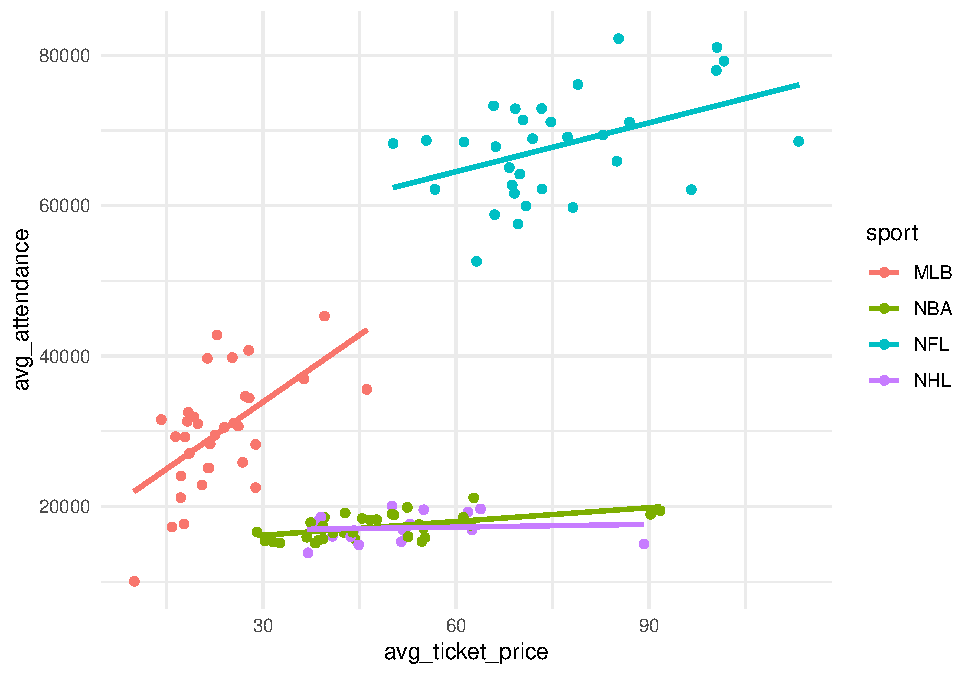
\includegraphics{Final_Project_files/figure-latex/tidy-1.pdf}

\begin{Shaded}
\begin{Highlighting}[]
\NormalTok{sports_rev }\OperatorTok
\StringTok{  }\KeywordTok{filter}\NormalTok{(sport }\OperatorTok{==}\StringTok{ "MLB"}\NormalTok{) }\OperatorTok
\StringTok{  }\KeywordTok{ggplot}\NormalTok{(}\KeywordTok{aes}\NormalTok{(avg_homewins, avg_attendance)) }\OperatorTok{+}
\StringTok{  }\KeywordTok{geom_point}\NormalTok{() }\OperatorTok{+}
\StringTok{  }\KeywordTok{geom_smooth}\NormalTok{(}\DataTypeTok{se =} \OtherTok{FALSE}\NormalTok{) }
\end{Highlighting}
\end{Shaded}

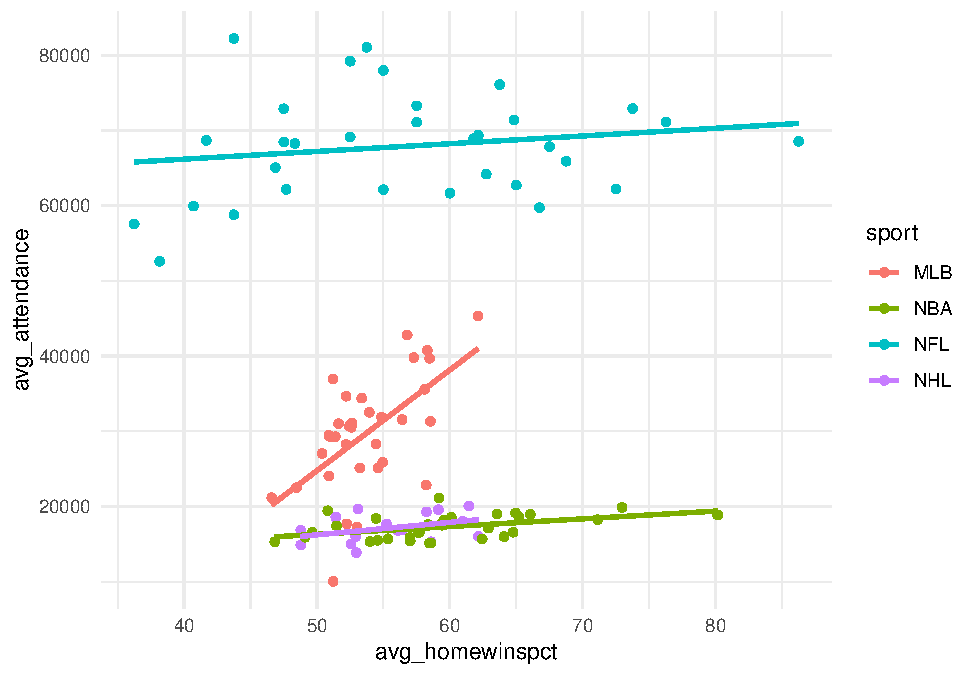
\includegraphics{Final_Project_files/figure-latex/tidy-2.pdf}

\begin{Shaded}
\begin{Highlighting}[]
\NormalTok{sports_pivot <-}\StringTok{ }\NormalTok{sports }\OperatorTok
\StringTok{  }\KeywordTok{pivot_longer}\NormalTok{(home_wins, }\DataTypeTok{names_to =} \KeywordTok{c}\NormalTok{(}\StringTok{"home"}\NormalTok{, }\StringTok{"wins"}\NormalTok{), }\DataTypeTok{names_sep =} \StringTok{"_"}\NormalTok{, }\DataTypeTok{values_to =} \StringTok{"victory"}\NormalTok{) }\OperatorTok
\StringTok{  }\KeywordTok{pivot_wider}\NormalTok{(}\DataTypeTok{names_from =}\NormalTok{ wins, }\DataTypeTok{values_from =}\NormalTok{ victory) }\OperatorTok
\StringTok{  }\KeywordTok{select}\NormalTok{(}\OperatorTok{-}\KeywordTok{c}\NormalTok{(}\DecValTok{9}\NormalTok{)) }\OperatorTok
\StringTok{  }\KeywordTok{rename}\NormalTok{(}\DataTypeTok{home_wins =}\NormalTok{ wins)}
\end{Highlighting}
\end{Shaded}

\hypertarget{requirements}{%
\subsection{Requirements}\label{requirements}}

\begin{enumerate}
\def\labelenumi{\arabic{enumi}.}
\tightlist
\item
  pivot\_longer: Done
\item
  pivot\_wider: Done
\item
  group\_by: Done
\item
  summarize: Done
\item
  filter: Done
\item
  select: Done
\item
  Mutate: Done
\end{enumerate}

\hypertarget{methods}{%
\section{Methods}\label{methods}}

We report how we determined our sample size, all data exclusions (if any), all manipulations, and all measures in the study.

\hypertarget{participants}{%
\subsection{Participants}\label{participants}}

\hypertarget{material}{%
\subsection{Material}\label{material}}

\hypertarget{procedure}{%
\subsection{Procedure}\label{procedure}}

\hypertarget{data-analysis}{%
\subsection{Data analysis}\label{data-analysis}}

We used R (Version 3.6.1; R Core Team, 2019) for all our analyses.

\hypertarget{results}{%
\section{Results}\label{results}}

\hypertarget{discussion}{%
\section{Discussion}\label{discussion}}

\newpage

\hypertarget{references}{%
\section{References}\label{references}}

\begin{Shaded}
\begin{Highlighting}[]
\KeywordTok{r_refs}\NormalTok{(}\DataTypeTok{file =} \StringTok{"r-references.bib"}\NormalTok{)}
\end{Highlighting}
\end{Shaded}

\begingroup
\setlength{\parindent}{-0.5in}
\setlength{\leftskip}{0.5in}

\hypertarget{refs}{}
\leavevmode\hypertarget{ref-R-base}{}%
R Core Team. (2019). \emph{R: A language and environment for statistical computing}. Vienna, Austria: R Foundation for Statistical Computing. Retrieved from \url{https://www.R-project.org/}

\endgroup


\end{document}
